\section{Spannungsversorgung}\label{sec.spannungsversorgung}
In diesem Abschnitt soll auf die hardwareseitige Umsetzung der Spannungsversorgung für die Wetterstation eingegangen werden. Ziel ist der Entwurf einer Platine, auf der sämtliche Anforderungen umgesetzt werden.

\subsection{Anforderungen}\label{subsec.anforderungen}
Zunächst sollen in diesem Abschnitt die Anforderungen, die sich aus der Aufgabenstellung ableiten lassen, sowie solche, die sich aus den weiteren Überlegungen zur Umsetzung der Wetterstation ergeben.

\begin{itemize}

	\item Messung des Ladestroms
	\item Messung der Batteriespannung (Ladezustand)
	\item Messung des Stromverbrauchs der Wetterstation

\end{itemize}

Des Weiteren soll der Stromverbrauch der Wetterstation so niedrig wie möglich sein, um die Puffer-Batterie zu schonen und sonnenarme Phasen bzw. die Nacht ohne Stromausfall überbrücken zu können. Die verwendete Batterie hat eine Ladeschlussspannung von 12\,V. Da für den Mikrocontroller und die Sensoren allerdings Spannungspegel von 3,3\,V und 5\,V benötigt werden, müssen diese auf der Platine erzeugt werden.

Aus den mechanischen Anforderungen, dass Mikrocontroller, Platine und Sensoren möglichst in einem Gehäuse untergebracht werden sollen, ergibt sich, dass die entworfene Platine auf die Pinheader des Mikrocontrollers gesteckt werden soll.

\subsection{Erzeugung benötigter Spannungen}\label{subsec.Spannungserzeugung}
Wie in \ref{subsec.anforderungen} beschrieben, werden sowohl 3,3V als auch 5V-Pegel für die Wetterstation benötigt. Angestrebt ist, dass die verwendeten Buck-Spannungsregler eine möglichst geringe Ruhestromaufnahme und einen guten Wirkungsgrad haben. Die Wahr fiel hierbei auf den \textit{LTC3621}. Dieser hat einen Eingangsspannungsbereich von 2,7\,V bis 17\,V und eine Ausgangsspannung, die sich über einen Spannungsteiler am Feedback-Pin zwischen 0,6\,V und der Eingangsspannung einstellen lässt. Der Ruhestrom beträgt laut Datenblatt 3,5\,$\mu$A ~\cite{ltc3621}. Der Regler kann einen maximalen Ausgangsstrom von 1\,A liefern. Da bei der Wahl des Spannungsreglers noch keine Werte über die von der Peripherie benötigte Leistung vorlag, ist dieser Wert eventuell etwas überdimensioniert.

Die Beschaltung des Reglers entspricht den Empfehlungen des Datenblatts und wird im folgenden Abschnitt dargestellt.


\subsubsection{3V3}\label{subsubsec.3v3}
Im folgenden soll hauptsächlich auf die Dimensionierung des Spannungsteilers zur Erzeugung von 3,3\,V eingegangen werden.

\subsubsection{5V}\label{subsubsec.5v}

\subsection{Spannungsabschaltung}\label{subsec.Spannungsabschaltung}

\subsection{Messung Strom/Spannung}\label{subsec.MessungStromSpannung}

\subsection{Beschaltung Sensoren}\label{subsec.BeschaltungSensoren}



%\begin{figure}[hbtp]
%  \centering
%  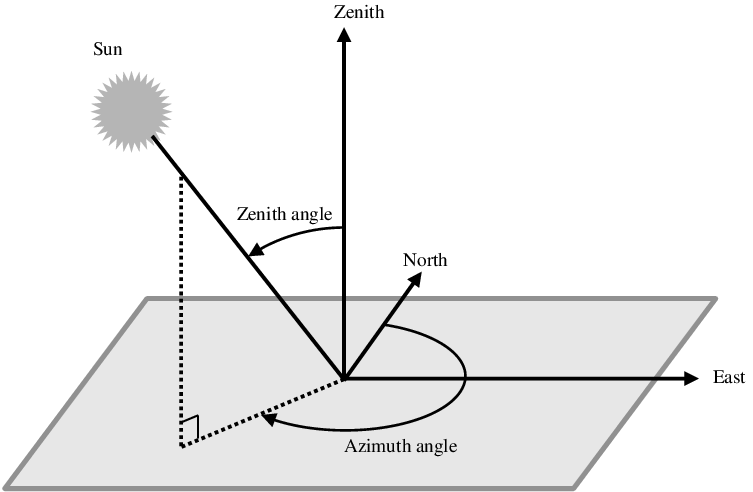
\includegraphics[width=\textwidth]{./img/Representation-of-azimuth-and-zenith-angles.png}
%  \caption{Beschreibung der Sonnenposition durch Zenith und Azimut~\cite{Nou2016}}\label{fig:zen_azi}
%\end{figure}